\documentclass[tikz, border=10pt]{standalone}
\usepackage{amsmath}
\usetikzlibrary{positioning}

\begin{document}
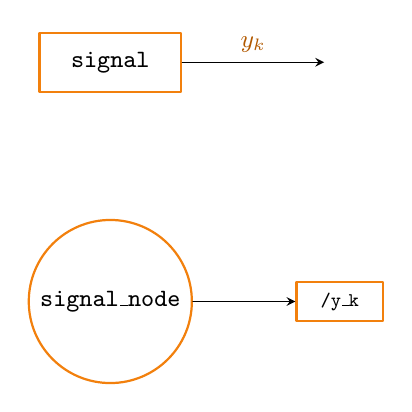
\begin{tikzpicture}[>=stealth, line cap=round, line join=round]

  % ── DynamicalSystem block (row b style) ──────────────────────────────────

  \node[draw=orange!80!brown, thick,
        minimum width=1.8cm, minimum height=0.75cm,
        font=\small\ttfamily] (sig) at (0, 0) {signal};

  \draw[->] (sig.east) -- ++(1.8, 0)
    node[midway, above, font=\small\itshape, orange!70!black] {$y_k$};

  % ── ROSNode circle (row c style) ──────────────────────────────────────────

  \node[draw=orange!80!brown, thick, circle,
        font=\small\ttfamily,
        below=1.6cm of sig] (signode) {signal\_node};

  % Output topic box
  \node[draw=orange!80!brown, thick,
        minimum width=1.1cm, minimum height=0.5cm,
        font=\scriptsize\ttfamily,
        right=1.3cm of signode] (topic) {/y\_k};

  \draw[->] (signode.east) -- (topic.west);

\end{tikzpicture}
\end{document}
